\section{Conversor digital a analógico (DAC)}

    Para controlar el voltaje de salida del convertidor reductor es necesario
    poder generar un voltaje de control de forma digital. Para ello se diseñó
    un conversor digital a analógico (DAC) utilizando un filtro RC de primer
    orden y un amplificador operacional en modo seguidor de voltaje. El DAC
    propuesto se muestra en la figura \ref{fig:dac}.

    \begin{figure}[H]
        \centering
        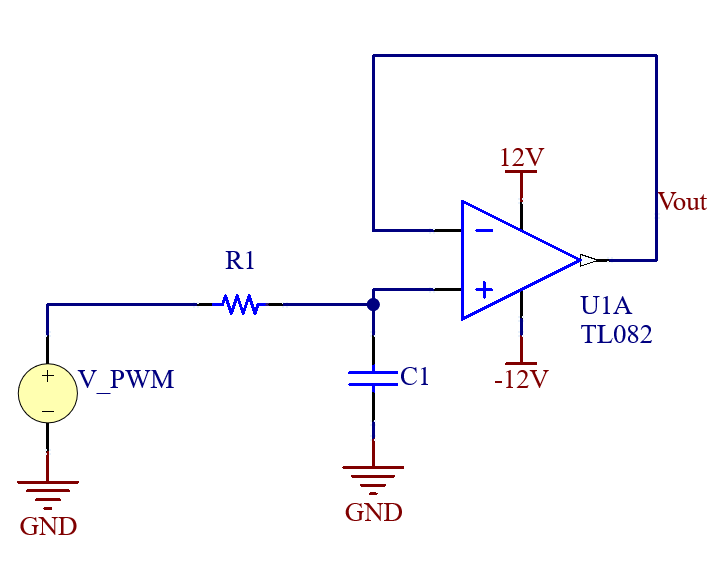
\includegraphics[scale=0.5]{imagenes/dac_disenio.png}
        \caption{DAC propuesto}
        \label{fig:dac}
    \end{figure}

    Ya que para la generación de la de PWM se utilizó el módulo PWM1 (debido
    a que este es el que presenta una mayor resolución) del ATmega328p, con el 
    cual se puede generar una señal PWM con una resolución de 10 bits, que en
    conjunto con una frecuencia de operación para el microcontrolador de $8\text{MHz}$
    se obtiene una frecuencia de PWM de $7.81\text{KHz}$, se determinó que la 
    frecuencia de corte del filtro RC sea de $70\text{Hz}$, de forma el armónico
    de mayor magnitud (el cual es el de frecuencia $7.81\text{KHz}$) sea atenuado
    en $-40\text{dB}$. 

    La frecuencia de corte para el filtro RC está dada por la ecuación \ref{eq:fc_dac},
    donde $R$ es el valor de la resistencia y $C$ es el valor del capacitor, mostrados
    en la figura \ref{fig:dac}.

    \begin{equation}
        f_c = \frac{1}{2\pi RC}
        \label{eq:fc_dac}
    \end{equation}

    Se fijó el valor del capacitor en $0.1\mu\text{F}$, por lo que el valor de la
    resistencia es de $22.7\text{K}\Omega$, por lo que se utilizará el valor 
    de resistencia comercial más cercano, el cual es de $22\text{K}\Omega$.
    Este cambio realizado en valor de la resistencia no afecta
    significativamente el comportamiento del filtro, ya que el objetivo 
    principal del mismo es atenuar los armónicos de la señal PWM, que es 
    dos órdenes de magnitud mayor a la frecuencia de corte del filtro.

    \subsection{Simulación del DAC}

    Para comprobar el correcto funcionamiento del DAC diseñado se realizó una
    simulación del mismo. Para ello se empleó el simulador LTspice, junto con
    el modelo spice proporcionado por texas instruments para el circuito integrado
    TL082 (descarga disponible en \cite{noauthor_tl082_nodate}). Para ello se 
    generó una señal pwm de $15.625KHz$ la cual varía su ciclo de trabajo 
    de forma que en la salida se obtenga una señal senoidal de $10\text{Hz}$. 
    En la figura
    \ref{fig:sim_dac} se muestra la respuesta del DAC ante la señal PWM de entrada.

    \begin{figure}[H]
        \centering
        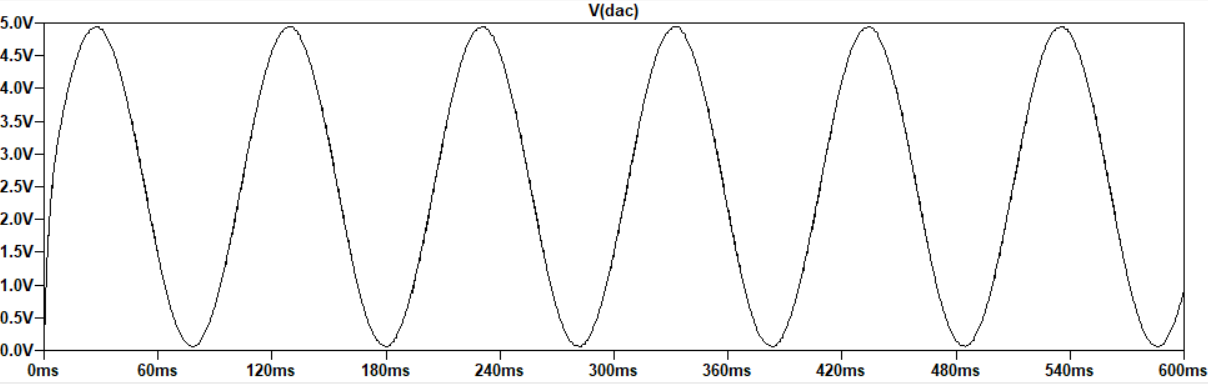
\includegraphics[scale=0.45]{imagenes/dac_out.png}
        \caption{Respuesta del DAC ante una señal PWM}
        \label{fig:sim_dac}
    \end{figure}

    En la figura \ref{fig:sim_dac} se puede observar que la señal de salida
    del DAC es una señal senoidal de $10\text{Hz}$, que es lo esperado ya 
    que la señal PWM varía su ciclo de trabajo también de forma senoidal.
    Además, se puede observar que el valor máximo de la señal de salida es
    de $5\text{V}$, mientras que el valor mínimo es cercano $0\text{V}$
    comprobando que el DAC funciona de forma correcta, ya que la señal PWM
    varía su ciclo de trabajo entre $0\%$ y $100\%$, haciendo que el valor 
    DC de la señal PWM varíe también entre $0\text{V}$ y $5\text{V}$.

    Adicionalmente en las figuras \ref{fig:sim_dac_fft} y \ref{fig:sim_dac_fft_in}
    se muestra la transformada de Fourier discreta (DFT) de la señal de salida
    del DAC, y de la señal PWM de entrada respectivamente. Se puede ver 
    que los armónicos correspondientes a la señal PWM de entrada son atenuados
    hasta el punto de que no son visibles en la DFT de la señal de salida del
    DAC, lo cual es lo esperado, ya que el filtro RC tiene una frecuencia de corte
    de $72\text{Hz}$, mientras que la frecuencia de la señal PWM es de 
    $15.625\text{KHz}$.

    \begin{figure}[H]
        \centering
        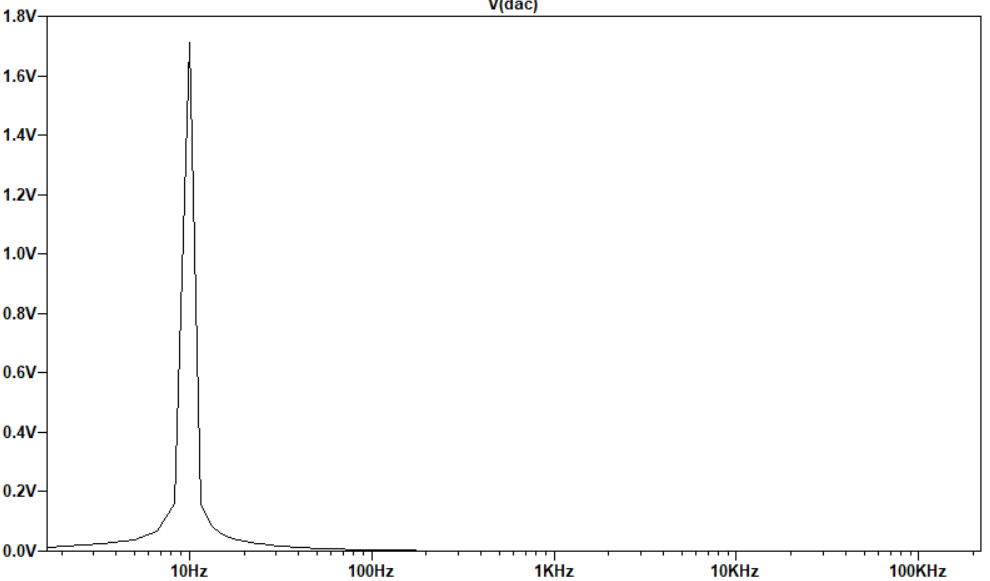
\includegraphics[scale=0.45]{imagenes/fft_dac_salida.png}
        \caption{DFT de la señal de salida del DAC}
        \label{fig:sim_dac_fft}
    \end{figure}

    \begin{figure}[H]
        \centering
        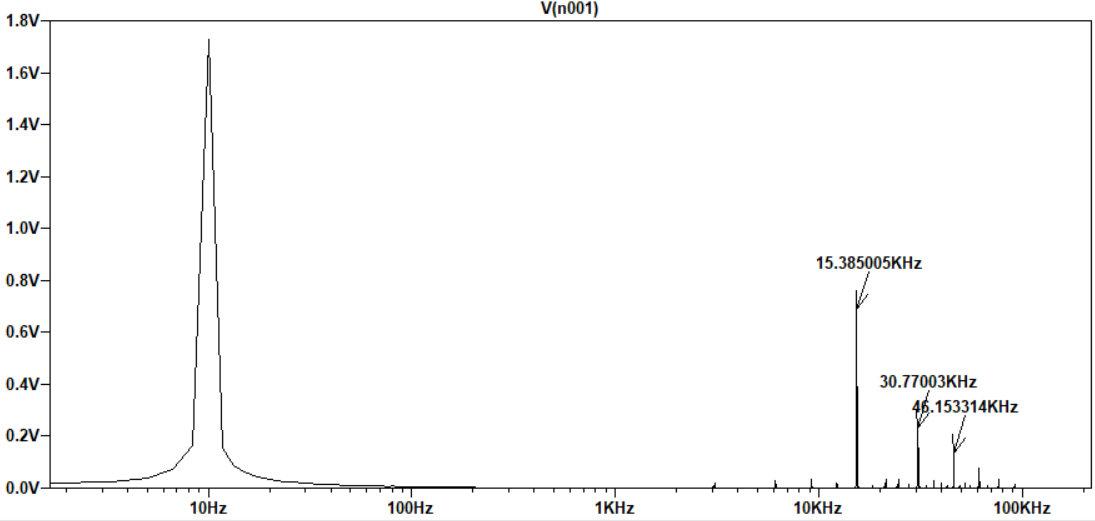
\includegraphics[scale=0.45]{imagenes/fft_dac_pwm.png}
        \caption{DFT de la señal PWM de entrada}
        \label{fig:sim_dac_fft_in}
    \end{figure}

    \subsection{Pruebas con DAC}

    Para comprobar el correcto funcionamiento del DAC diseñado se realizó una
    prueba del DAC, en la cual se generaró 2 señales, una senoidal y una triangular,
    empleando el DAC y el codigo mostrado en el apéndice \ref{sec:codigo_dac} (el cual 
    se puede ubicar dentro de los archivos del proyecto de MPLAB nombrado como
    DAC\_test.X, dentro de la carpeta nombrada Charge\_system\_firmware).
     En la figura \ref{fig:dac_test_sine}
    se muestra el resultado de la prueba.
    
     \begin{figure}[H]
        \centering

        \begin{subfigure}{0.45\textwidth}
            \centering
            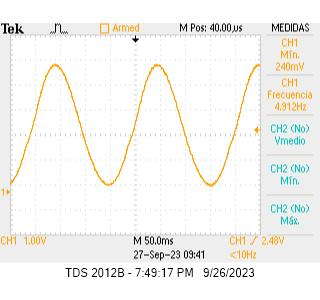
\includegraphics[scale=0.8]{imagenes/Sine.jpg}
            \caption{Señal senoidal}
        \end{subfigure}
        \begin{subfigure}{0.45\textwidth}
            \centering
            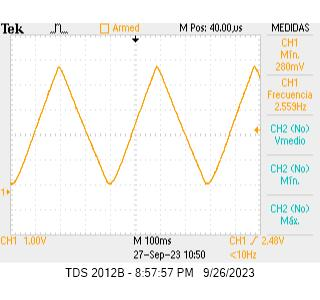
\includegraphics[scale=0.8]{imagenes/Triangular.jpg}
            \caption{Señal triangular}
        \end{subfigure}

        \caption{Señal seno y triangular generadas con el DAC}
        \label{fig:dac_test_sine}
     \end{figure}

     Se puede observar que ambas señales
     tienen una amplitud de $5\text{V}$, y que la señal senoidal tiene una frecuencia
     de $4.91\text{Hz}$, mientras que la señal triangular tiene una frecuencia de
     $2.56\text{Hz}$. La razon por la cual las frecuencias de las señales generadas
     son bajas es debido a la frecuencia de corte del filtro RC, que es de $72\text{Hz}$,
     por lo que señales de mayor frecuencia son atenuadas, hecho que no afecta 
     al sistema de carga multiquímica, ya que la el cambio de voltaje de voltaje 
     en ambas baterias se realiza de forma lenta, por lo que no es necesario
     generar señales de alta frecuencia.
 